\documentclass{report}
\usepackage[francais]{babel}
\usepackage[utf8]{inputenc}
\usepackage{graphicx}


\begin{document}
\begin{titlepage}

\title{\Huge CoMFoRT \\
       \huge Manuel d'utilisation}
\author{Projet2 de L3IF -- \texttt{comfort@listes.ens-lyon.fr}}
\date{2008}
\begin{figure}
\begin{center}
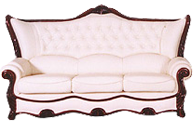
\includegraphics{confort.png}
\end{center}
\end{figure}
\end{titlepage}
  \maketitle

  \tableofcontents
\chapter{Installation}

    \paragraph{}Il est possible d'installer CoMFoRT sous Linux, Mac ou
	Windows.
	\`A noter que Python s'installera en m\^eme temps que notre CMS s'il
	n'est pas déjà présent sur la machine... Il est un petit peu essentiel.
  \section{Linux}
    Il suffit d'installer le paquet Debian \texttt{comfort}.
  \section{Windows}
    \paragraph{} Pour installer CoMFoRT sous Windows, il suffit de lancer le
	programme d'installation et de suivre les instructions.

\chapter{Introduction à CoMFoRT}

Félicitations, vous venez d'installer CoMFoRT~! 

En lançant le logiciel vous
arrivez sur une page vous demandant quelques informations, telles que le
titre de votre site ou encore l'adresse FTP de votre futur site. 

Une fois ces informations remplies vous arrivez sur la page d'accueil de votre futur
site. Cette page contient une brève introduction à l'utilisation de CoMFoRT
qui sera par la suite effacée afin de laisser place à votre page d'accueil.

Il y a aussi une seconde page qui explique la syntaxe wiki utilisée. 
Cette page est supprimable. 

La première action à
réaliser est de cliquer sur le bouton "Panneau d'administration" situé en
bas de la page. Le panneau d'administration va permettre de gérer l'ensemble
de votre site. Il se décompose en trois parties~: "Configuration générale",
"Configuration des modules" et "Travail en local". 
\begin{itemize}
\item La première sert à la
gestion de la structure du site, telle que le thème ou la gestion des pages.
\item La seconde sert à la gestion du contenu à l'aide des modules dont nous
verrons l'usage plus bas. 
\item La dernière partie sert quant à elle à la mise en
ligne des modification et à l'arrêt du logiciel.
\end{itemize}
\chapter{Gestion des pages}

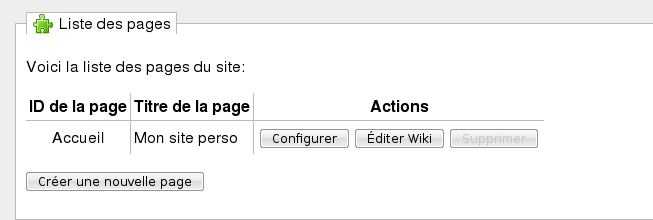
\includegraphics[width=14cm,height=4cm]{capture16.png}

  \section{Créer/Supprimer des pages}
     \paragraph{}Au départ, le site ne comporte qu'une unique page : la page
	 d'accueil, page qu'il est possible de modifier de la même manière que
	 les autres mais que l'on ne peut pas supprimer. 
	 
	 Il est possible de
	 rajouter autant de pages que l'on veut, la seule contrainte étant que
	 chacune d'entre elles doit avoir un nom différent. 
	 
	 Par défaut, seuls
	 les modules "menu" et "wiki" sont actifs sur une nouvelle page.
    \paragraph{Parenthèse sur les modules} La partie "texte" d'une page est
	gérée via un système de wiki dont la syntaxe est décrite plus bas. Mais
	pour plus de simplicité et d'efficacité certaines parties précises sont
	gérées via ce que l'on nomme un module. Il s'agit d'un bloc
	d'informations particulières, comme l'ensemble de vos publications.
	L'activation d'un module sur une page est donc l'importation des
	informations de ce module sur la page. Par exemple en activant le module
	"Publication" la page va contenir la liste de toutes vos publications.
    \paragraph{Création} On peut créer autant de pages que l'on veut à
	partir de la page administrateur en utilisant la commande "créer une
	nouvelle page". Lors de la création, on paramètre la page à volonté
	(identifiant unique, titre) puis on choisit les modules que l'on souhaite 
	activer sur la page en les ordonnant selon ses besoins. Si le module "wiki"
	est	activé on va ensuite pouvoir éditer le wiki de la page bien que rien ne
	soit définitif, une page étant modifiable à souhait.
    \paragraph{Suppression}Pour supprimer une page, il suffit de cliquer sur
	le bouton correspondant. \`A noter que la page d'accueil ne peut pas
	être supprimée.
    \paragraph{Insertion d'une page générée en dehors de CoMFoRT} Il est
	possible d'ajouter une page générée indépendamment de notre CMS. Pour
	cela il suffit de l'ajouter dans le dossier ~/.comfort/perso/pages
	générées, elle sera alors téléchargée vers le serveur avec les autres.
  \section{Modifier une page}
     \paragraph{Modification}Chaque page est entièrement paramétrable~: il
	 suffit de cliquer sur la commande "configurer" pour activer ou
	 désactiver des modules, et sur "édition du wiki" pour modifier ce
	 dernier selon nos souhaits (par exemple pour supprimer le texte
	 d'introduction de la page d'accueil).
     \paragraph{Mise en ligne}Toutes les modifications apportées sont faites
	 en local. Une fois le site mis à jour en local, il ne reste plus qu'à
	 le générer et à l'envoyer sur le serveur. Avant cette opération, aucune
	 modification n'est enregistrée, ni publiée.


\chapter{Gestion des publications}

CoMFoRT étant orienté vers les chercheurs, il propose une gestion efficace
des publications.
  \section{Import}
Il vous permet d'importer les informations sur vos publications de
différentes fa\c{c}ons :
\begin{itemize}
 \item{Vous pouvez bien entendu les fournir "à la main" via un formulaire}
 \item{Mais vous pouvez aussi fournir un fichier BiBTeX, et CoMFoRT se
 charge alors d'extraire les informations utiles.}
 \item{(À venir) Et finalement, vous pouvez également importer les
 informations sur vos publications de manière automatique en fournissant
 uniquement votre nom. CoMFoRT se charge alors d'aller chercher les
 informations via Google Scholar, et vous demande uniquement de
 sélectionner quelles publications sont bien les v\^otres.}
\end{itemize}

  \section{Export}
Vous pouvez également exporter en BiBTeX la liste des publications que vous
avez rajoutées au site, et même sélectionner juste une partie de ces
publications (par exemple celles de l'année écoulée). Cela vous permet par
exemple d'importer toutes les informations nécessaires sur vos publications
sur le site HAL du CNRS ou de l'INRIA.
  \section{Gestion de la liste des publications}
Vous pouvez également gérer vos publications en les groupant sous forme de
liste. Ce regroupement sous forme de liste va permettre de trier les
publications de la manière que l'on veut ou même de n'afficher qu'une partie
des publications.

\chapter{Personnalisation du site}

  \section{Thèmes}
    \paragraph{}CoMFoRT propose un thème par défaut. Il est toutefois
	possible d'en choisir un autre facilement. Ainsi il est proposé une
	bibliothèque de thèmes prédéfinis qui se situe dans la partie
	"configuration du site" du panneau d'administration ("feuille de style à
	utiliser"). Il est aussi possible d'en importer, d'en créer de nouveaux
	ou d'en modifier des préexistants.
    \paragraph{Créer/Ajouter un thème} 
      \begin{itemize}
        \item Créer un dossier dans /src/styles
	\item Mettre dans ce dossier la feuille de style CSS correspondante et
	les éventuelles images utilisées par le fichier CSS. Pour la création de
	thème, il est suggéré de s'inspirer des feuilles de style préexistantes.
      \end{itemize}

  \section{Modules}
    \label{Modules}
    \paragraph{Activation des modules}Par défaut, seuls les modules "menu" et
	"wiki" sont activés sur une page. Pour en activer d'autres, il faut se
	rendre dans la page d'administration et activer les modules désirés
	suivant les pages. Les autres modules disponibles sont : "news",
	"calendrier", "enseignements", "publications", "agenda".
    \paragraph{Agencement des modules}L'ordre des modules sur la page
	administrateur est l'ordre dans lequel seront affichés tous les modules
	dans CoMFoRT. Ceci est réglable~: on peut monter/descendre un module.
  \section{Module wiki}
    \paragraph{Pourquoi un module wiki} Le module "wiki" est un module dont le
	r\^ole premier est de permettre à l'utilisateur de s'exprimer comme il
	le désire. Il vient en complément des autres modules et il peut servir à
	remplir des fonctions que ne remplirait pas un des autres modules. Il ne 
	peut cependant y avoir qu'un seul module "wiki" par page.
    \paragraph{Syntaxe}On utilise comme syntaxe, dans le module "wiki", un
	sous-ensemble de la syntaxe de Wikipédia. 
	Syntaxe supportée :
	\begin{itemize}
	  \item \textbf{Paragraphes :} pour passer au paragraphe suivant, il
	  faut sauter une ligne.
 
	  \item \textbf{Titres :}  ==, ===, ====, ===== et ======.
		 
		 Ex: \verb|== Titre ==|
	  \item \textbf{Formatage :} 

		\begin{itemize}
		  \item \textbf{italique :} \verb|''|
                  Ex: \verb|''italique''|
		  \item \textbf{gras :} \verb|'''|
				  Ex: \verb|'''gras'''|
		  \item \textbf{italique + gras :} \verb|'''''|
				  Ex: \verb|'''''italique ET gras'''''|
		\end{itemize}
	  \item \textbf{Taille du texte :}
		\verb|<small>text</small>| affiche le texte en petit et inversement
		pour \verb|<big>|.
	  \item \textbf{Liens :} Pour un lien vers un élément interne à CoMFoRT, la
	  syntaxe est \verb|[[lien]]|, pour un élément externe \verb|[lien]|.
		\begin{itemize}
		  \item Lien hypertexte: 
			\verb?[url|texte]? 
			équivalent à 
			\verb|<a href="url">texte</a>|
                     le champ texte peut \^etre omis, dans ce cas, il vaut url
                     idem pour les liens internes avec \verb|[[]]| (dans ce cas
                     "url" doit être l'identifiant de la page).
		  \item Image: Syntaxe:
		  \begin{verbatim}[[Image:url|thumb|position|taille|légende]]\end{verbatim}
		  Les champs thumb, position, taille et légende peuvent \^etre omis.
			\begin{itemize}
			  \item \verb|url|: url de l'image
			  \item \verb|position|: vaut left,center ou right
			  \item taille: syntaxe: 
				  \begin{itemize}
					\item \verb|300px|: l'image fait 300 pixels de large ou de
					haut (suivant la dimension la plus grande de l'image)
					\item \verb|300|: idem
					\item \verb|300x200px|: l'image fait 300 pixels de large,
					200 de haut
				  \end{itemize}
			  \item \verb|légende|: texte affiché si l'image ne peut pas \^etre chargée
			  \item \verb|thumb|: si précisé, équivalent à indiquer pour la taille: 180px
				
				\verb?[[Image:coucou.gif|thumb]]? équivalent
				\verb?[[Image:coucou.gif|180px]]?
				idem pour les images externes avec \verb|[]|.
			\end{itemize}
		  \item Lien vers une page perso:
			\verb?[[Page:url|texte]]? idem que les liens hypertextes: url est
			l'url est le chemin relatif dans perso/pages
		  \item Lien vers une image perso:
			\verb?[[Picture:url|texte]]? idem que les liens hypertextes: url est l'url est le
			chemin relatif dans perso/pictures
		  \item Lien vers une doc perso:
			\verb?[[Doc:url|texte]]? idem que les liens hypertextes: url est l'url est le
			chemin relatif dans perso/docs
		\end{itemize}
	  \item \textbf{Exposants :} \verb|{{exposant}}| ou \verb?{{exp|exposant}}? ou
	  \verb|<sup>exposant</sup>|
	  \item \textbf{Indices :} \verb|{{indice}}| ou \verb?{{ind|indice}}? ou
	  \verb|<sub>indice<sub>|
	  \item \textbf{Tableaux :} 
		\begin{verbatim}
		{|        :   début du tableau
		|+ titre  :   ajoute un titre au tableau
		|-        :   ajoute une nouvelle ligne
		| texte   :   ajoute une nouvelle cellule dans la ligne courante contenant texte
		| options | texte : idem que ci-dessus avec les options ci-dessus en plus:
                     * align="left"|"center"|"right"
                     * valign="top"|"middle"|"bottom"
                     * colspan=x: la case s'étend sur x colonnes
                     * rowspan=x: la case s'étend sur x lignes
		|}        : fin de tableau
		\end{verbatim}
	  \item \textbf{Listes :} 
		\begin{itemize}
		  \item Les listes non ordonnées:
			  En début de ligne:  * crée une nouvelle puce
			  Exemple:
				\begin{verbatim}
				* puce numéro 1
				* puce numéro 2
				* puce numéro 3
				\end{verbatim}
		  \item Les listes ordonnées:
  En début de ligne:  \# crée un nouvel item pour une liste numérotée
  Exemple:
	  \begin{verbatim}
	  # item 1
	  # item 2
	  
	  sortie -->   1. item 1
	               2. item 2
	  \end{verbatim}
		  \item On peut mixer les deux:
  
  Exemple 1:
  \begin{verbatim}
    * puce 1
    * puce 2
    # item 1
    # item 2
  
    sortie -->   * puce 1
                 * puce 2
                   1. item 1
                   2. item 2
  \end{verbatim}
  
  Exemple 2:
  \begin{verbatim}
    * une liste
    # item 1
    ## item 11
    ** coucou
    ### item 111
    ## item 12
    # item 2

    sortie -->   * Une liste
                      1. item 1
                         a. item 11
                            * coucou
                         b. item 12
                      2. item 2
  \end{verbatim}
		\end{itemize}
	  \item \textbf{Texte préformaté :} ajouter un espace en début de ligne.
	  \item \textbf{Balises :} 
		\begin{itemize}
		  \item math: insère du latex dans le wiki
    
		  \verb|<math size="x" packages="p">code latex</math>|
		  \begin{itemize}
			\item \verb|x|: la taille du latex (par défaut: 200)
			\item \verb|p|: les paquets à utiliser sous la forme 
			"paquet1 paquet2 paquet3..."
		  \end{itemize}
		  \item nowiki: \verb|<nowiki>text</nowiki>| insère text tel quel
		  dans le wiki sans le modifier.
		  \item h2, h3, h4, h5 et h6:  \verb|<h2>Titre</h2>| équivaut à
		  \verb|==Titre==|
                           idem pour h3 et ===, etc...
		  \item ul, ol et li: balises pour les listes, idem qu'en XHTML
		  \item ref: \verb|<ref>référence</ref>| insère une note de bas de page avec comme texte "référence"
		  \item sup et sub: cf exposant et indice
		  \item pre: \verb|<pre>texte</pre>| insère du texte préformaté,
		  idem que espace en début de ligne
		  \item i, b, u, s, center et highlight: balise italique, gras, souligné,
		  barré, centré et sur-ligné
		  \item \verb|</br>| va à la ligne
		  \item \verb|<module />|:

		  \verb|<module id="mod" params="key1=value1&key2=value2..." />|
		  insère le contenu du module "mod" appelé avec les arguments 
		  
		  \verb|{key1: value1, key2: value2, ...}|
		\end{itemize}
	\end{itemize}

	Syntaxe prise en charge mais sans effet:
    \begin{itemize}
	  \item le \verb|:| en début de ligne, censé faire des tabulations
	  \item le \verb|</hr>| : insère un séparateur
	  \item le \verb|!| en début de ligne dans un tableau: m\^eme effet que
	  le \verb?|?
    \end{itemize}

  \section{Les autres modules}
   \paragraph{Les news et le calendrier}Ces modules permettent d'afficher
   sur les pages de votre site une liste de news ou d'évènements à venir que
   vous aurez préalablement fournie. Pour ajouter une news il suffit
   d'appuyer sur le bouton correspondant et de remplir les informations que
   l'on souhaite voir apparaître. Le module Calendrier fonctionne de la même
   manière.
   \paragraph{Le menu}Ce module permet juste d'afficher les boutons d'accès
   aux pages lorsqu'il est activé.
   \paragraph{Enseignement}Il fonctionne de la même manière que les autres,
   on ajoute un enseignement en donnant les informations correspondantes.
   Mais une fois un enseignement crée on peut lui adjoindre des documents et
   une bibliographie (une liste parmi celles que l'on a crées).

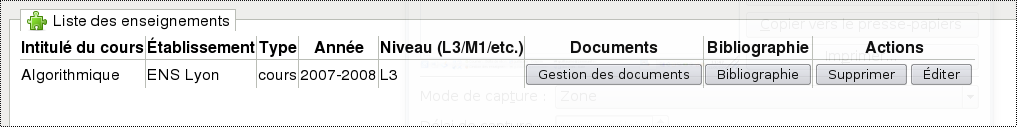
\includegraphics[width=16cm,height=3cm]{capture22.png}

  \section{Ajout d'un module}
    \paragraph{Comment ajouter un module}Pour ajouter un module, vous pouvez
	vous baser sur les modules déjà existants. Dans
	\verb|modules\_interfaces.py|, vous trouverez différentes interfaces que 
	vous pouvez choisir	d'implémenter~:
    \begin{itemize}
      \item IModuleAdminPage pour les modules utilisant une page de
	  configuration dans la partie administration. Vous pourrez par exemple
	  vous baser sur le modules "News" pour vous familiariser avec
	  l'écriture de formulaires pour l'administration, et la gestion des
	  valeurs de retour ainsi que l'insertion dans la base de données\dots
      \item IModuleDB pour les modules utilisant la base de données (la
	  méthode \verb|setup\_db| permet de récupérer l'objet db sur lequel on
	  peut effectuer les requ\^etes).
      \item IModuleContentProvider pour les modules fournissant du contenu
      \item les autres interfaces ne sont pas encore utilisées à l'heure
	  actuelle.
    \end{itemize}
Ajouter un module consiste à ajouter un fichier
"\verb|themodule\_NomDeVotreModule.py|" dans le dossier modules, ce fichier
contenant une classe "TheModule" qui hérite des interfaces correspondant à
ce que fait le module.

  \section{Contacts}La classe de L3IF 07-08 a, dans le cadre du projet, une
  mailing list qui reste à votre disposition pour vous éclairer quant aux
  différentes particularités du projet et pour faire profiter les autres
  utilisateurs de vos contributions.

  \texttt{comfort@listes.ens-lyon.fr}


\end{document}
